% Tài liệu bổ sung của paper_vi/main_vi.tex. Bảng số sinh tự động bởi tables/make_tables.py (không sửa tay).
\documentclass[11pt,a4paper]{article}
\usepackage[utf8]{inputenc}
\usepackage[T5]{fontenc}
\usepackage[vietnamese]{babel}
\usepackage[margin=2.5cm]{geometry}
\usepackage{amsmath,amssymb,booktabs,array,graphicx,xcolor}
\usepackage[colorlinks=true,linkcolor=blue]{hyperref}
\graphicspath{{figures/}{./}}
\newcommand{\Ntau}{N_{\tau}}
\newcommand{\todo}[1]{\textcolor{red}{[TODO: #1]}}
\renewcommand{\thetable}{S\arabic{table}}
\renewcommand{\thefigure}{S\arabic{figure}}
\title{Tài liệu bổ sung: Tấn công cạn kiệt tài nguyên qua NMS có thực sự làm chậm bộ phát hiện? Một nghiên cứu đo lường trên CPU ghim lõi}
\date{}
\begin{document}
\maketitle

\section{Bộ tối ưu của nghiên cứu tình huống}
Quy trình tối ưu và đánh giá miếng dán được tóm tắt ở Bảng~\ref{tab:algo}; thiết lập của từng điều kiện ở bài chính. Fitness huấn luyện theo ngân sách (Bảng~\ref{tab:train}, Hình~\ref{fig:budget}) cho thấy thuật toán di truyền bão hòa sớm và không vượt tìm kiếm ngẫu nhiên cùng cách đặt vị trí; baseline gradient (hộp trắng) cao hơn xa mọi điều kiện không dùng gradient. Giá trị fitness phụ thuộc vào ngưỡng và kích thước đầu vào, nên chỉ so được trong cùng đầu vào và ngưỡng.

\begin{table}[h]
\centering\small
\caption{Quy trình tối ưu và đánh giá miếng dán.}
\label{tab:algo}
\begin{tabular}{@{}cp{12.5cm}@{}}
\toprule
Bước & Thao tác \\
\midrule
1 & Khởi tạo 20 tensor RGB; chọn vị trí theo chính sách (độ nổi bật, tâm hoặc ngẫu nhiên). \\
2 & Chèn từng cá thể vào các ảnh tối ưu. \\
3 & Lấy mẫu biến đổi; suy luận và đọc điểm tin cậy trước NMS. \\
4 & Tính fitness; ghi số lượt ảnh và cá thể tốt nhất. \\
5 & Giữ năm cá thể ưu tú; lai ghép ngang và đột biến để tạo 15 con. \\
6 & Dừng khi hết ngân sách lượt ảnh; khóa miếng dán và ghi giá trị băm. \\
7 & Đánh giá độc lập trên ảnh giữ ra ngoài. \\
\bottomrule
\end{tabular}
\end{table}

\begin{table}[t]
\centering\small
\caption{Fitness huấn luyện (trung bình trên mười seed, độ lệch chuẩn trong ngoặc) ở ba mức ngân sách (lượt lan truyền thuận ứng viên--ảnh), trường \texttt{best\_training\_fitness} của checkpoint. Với B4, phương pháp gradient cập nhật một patch duy nhất nên giá trị là fitness ở bước cuối của mốc ngân sách.}
\label{tab:train}
\begin{tabular}{@{}lccc@{}}
\toprule
Điều kiện & 10\,000 & 25\,000 & 62\,500 \\
\midrule
C1 (320 px, $\tau_{\mathrm{obj}}$ 0,01) & 185,1 (1,7) & 185,9 (1,2) & 186,6 (1,6) \\
C3 (320 px, $\tau_{\mathrm{obj}}$ 0,25) & 39,8 (0,2) & 40,0 (0,3) & 40,5 (0,3) \\
C2 (640 px, patch 128 px) & 294,4 (3,9) & 295,5 (2,9) & 297,3 (2,2) \\
C4 (640 px, patch 64 px) & 299,4 (1,3) & 301,4 (1,9) & 303,1 (1,7) \\
B1 (đặt ở tâm) & 188,7 (1,5) & 189,8 (1,0) & 191,0 (1,4) \\
B2 (đặt ngẫu nhiên) & 191,6 (1,9) & 193,1 (1,5) & 193,5 (1,9) \\
B3 (tìm kiếm ngẫu nhiên) & 184,5 (0,8) & 185,1 (0,8) & 186,0 (1,0) \\
B4 (gradient, tanh) & 218,1 (14,9) & 314,4 (12,8) & 334,1 (11,6) \\
\bottomrule
\end{tabular}
\end{table}

\begin{figure}[h]
\centering
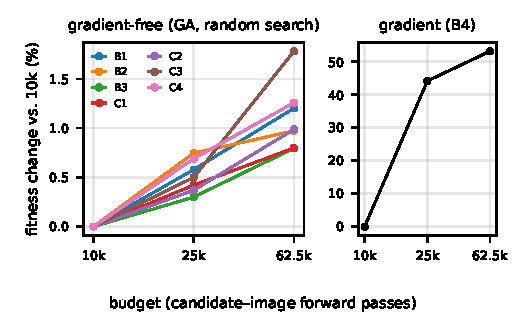
\includegraphics[width=0.8\textwidth]{fig7_training_budget.pdf}
\caption{Thay đổi fitness huấn luyện (trung bình mười seed) theo ngân sách, so với mốc 10\,000 lượt.}
\label{fig:budget}
\end{figure}

\section{Mô tả thêm của đối chứng dương}
Bảng~\ref{tab:slopes} cho độ dốc log--log của các đường cong đáp ứng liều; chỉ mang tính mô tả, không suy ra lớp độ phức tạp. Về số lớp: các cài đặt không phân biệt lớp không bị ảnh hưởng bởi số lớp, còn các cài đặt phân biệt lớp nhanh hơn khi chỉ có một lớp (số liệu: \texttt{contrasts.nc80\_over\_nc1} trong tệp tóm tắt của đối chứng dương).

\begin{table}[t]
\centering\small
\caption{Độ dốc log--log của độ trễ NMS theo $\Ntau$ trên các mức đã đo $\ge 100$ (head 10\,000 anchor, 80 lớp, không giới hạn); khoảng tin cậy bootstrap 95\% trong ngoặc. Chỉ mang tính mô tả.}
\label{tab:slopes}
\begin{tabular}{@{}lccc@{}}
\toprule
Cách cài đặt & Rời nhau & Cụm dày đặc & Hỗn hợp \\
\midrule
PyTorch thuần & 1,17 [1,17; 1,17] & 0,30 [0,29; 0,32] & 1,07 [1,05; 1,08] \\
torchvision \texttt{nms} & 1,59 [1,58; 1,60] & 0,69 [0,67; 0,69] & 1,42 [1,40; 1,45] \\
torchvision theo lô & 1,09 [1,08; 1,10] & 1,08 [1,07; 1,09] & 1,07 [1,05; 1,08] \\
Ultralytics gốc & 1,29 [1,29; 1,30] & 0,96 [0,95; 0,97] & 1,21 [1,20; 1,21] \\
\bottomrule
\end{tabular}
\end{table}

\section{Tỷ số NMS theo cách cài đặt cho từng patch}
\begin{table*}[t]
\centering\small
\caption{Tỷ số thời gian công đoạn NMS (đo vi mô, $\tau=0{,}01$) của ảnh có patch so với ảnh sạch cùng canvas, theo cách cài đặt; tỷ số trung bình, KTC 95\% bootstrap hai tầng. Cùng lần đo với bảng patch của bài chính; bước chèn patch nằm ngoài bộ đếm của công đoạn này.}
\label{tab:impl}
\begin{tabular}{@{}lcccc@{}}
\toprule
Điều kiện & PyTorch thuần & \texttt{nms} & Theo lô & Ultralytics \\
\midrule
C1 (320 px) & 1,065 (1,003--1,133) & 1,003 (0,987--1,018) & 1,000 (0,987--1,013) & 1,006 (0,991--1,023) \\
C3 (320 px) & 1,059 (0,997--1,126) & 1,010 (0,992--1,028) & 1,002 (0,987--1,018) & 1,004 (0,990--1,017) \\
B1 (320 px) & 1,066 (1,009--1,128) & 1,017 (0,998--1,037) & 1,002 (0,988--1,015) & 1,003 (0,989--1,016) \\
B2 (320 px) & 1,094 (1,052--1,143) & 1,022 (1,003--1,042) & 1,007 (0,994--1,020) & 1,009 (0,995--1,022) \\
B3 (320 px) & 1,066 (1,001--1,135) & 1,006 (0,988--1,023) & 0,996 (0,982--1,009) & 1,000 (0,986--1,014) \\
B4 (320 px) & 2,372 (2,096--2,674) & 1,228 (1,197--1,260) & 1,121 (1,101--1,141) & 1,126 (1,107--1,146) \\
C2 (640 px) & 1,100 (1,022--1,193) & 1,019 (0,989--1,048) & 1,021 (0,992--1,061) & 1,009 (0,986--1,030) \\
C4 (640 px) & 1,090 (1,046--1,143) & 1,032 (0,998--1,067) & 1,061 (1,015--1,141) & 1,019 (0,996--1,043) \\
\bottomrule
\end{tabular}
\end{table*}

\section{Lỗi chèn patch và lần đo lại bị loại}
Lần đo patch (studies/e6\_remeasure) gọi bước chèn patch bên trong bộ đếm toàn trình của nhánh có patch nhưng không ở nhánh sạch; bộ đếm của lọc điểm và NMS không bị ảnh hưởng. Lần đo lại với bước chèn ngoài vùng bấm giờ (studies/e11\_patch\_remeasure, có tệp đăng ký trước riêng) bị loại vì drift. Bài chính vì vậy không báo số toàn trình đo được của patch; cột toàn trình là dự đoán của mô hình ngân sách. Mọi bản ghi thô của cả hai lần đo được giữ trong kho mã.

\end{document}
